\documentclass[12pt,a4paper]{article}

\usepackage[a4paper,margin=2.5cm]{geometry}
\usepackage{iftex}
\ifXeTeX
  \usepackage{fontspec}
  \setmainfont{Liberation Serif}
  \setmonofont{DejaVu Sans Mono}
  \usepackage{polyglossia}
  \setmainlanguage{russian}
\else
  \usepackage[T2A]{fontenc}
  \usepackage[utf8]{inputenc}
  \usepackage[russian]{babel}
\fi
\usepackage{graphicx}
\usepackage{booktabs}
\usepackage{float}
\usepackage[hidelinks]{hyperref}
\usepackage{enumitem}

% ====== ПОДСТАВИТЬ ПЕРЕД СДАЧЕЙ ======
\newcommand{\repourl}{https://github.com/YOUR_LOGIN/secure-api}
\newcommand{\runurl}{https://github.com/YOUR_LOGIN/secure-api/actions/runs/XXXXXXXX}
\newcommand{\groupnum}{P3317}
% =====================================

\newcommand{\code}[1]{\texttt{\small #1}}
\setlist{itemsep=2pt,topsep=4pt}

\begin{document}

\begin{titlepage}
\thispagestyle{empty}

\begin{center}

\textbf{Федеральное государственное автономное
образовательное учреждение высшего образования
\\
«Национальный
исследовательский университет ИТМО»}\\[12pt]
Факультет программной инженерии и компьютерной техники\\
Направление подготовки: 09.03.04\\
Программная инженерия, Системное и прикладное программное обеспечение
\end{center}

\vspace*{4cm}

\begin{center}
\textbf{Отчёт}\\[4pt]
по лабораторной работе\\
по дисциплине «Информационная безопасность»\\[1em]
\textbf{Работа № 1}\\[4pt]
\textbf{«Разработка защищённого REST API с интеграцией в CI/CD»}
\end{center}

\vfill

\begin{flushright}
\textbf{Выполнил:}\\
Мищенко Роман Андреевич\\
Группа \groupnum\\[12pt]
\textbf{Преподаватель:}\\
Маркина Татьяна Анатольевна
\end{flushright}

\vfill

\begin{center}
Санкт-Петербург\\
2026
\end{center}

\end{titlepage}

\section{Ссылки на результаты}
\begin{itemize}
  \item Публичный репозиторий с кодом: \url{\repourl}
  \item Последний успешный запуск pipeline: \url{\runurl}
\end{itemize}

\section{Описание проекта и API}
Проект --- учебный backend на Python (Flask) с базой данных SQLite. Назначение --- показать, как защитить веб-API от
уязвимостей из OWASP Top 10 и встроить проверки безопасности в процесс разработки (CI/CD).

\begin{table}[H]
\centering\small
\begin{tabular}{llp{7.2cm}}
\toprule
Метод и путь & Доступ & Описание \\
\midrule
\code{POST /auth/login} & публичный & Принимает логин и пароль, при успехе возвращает JWT (срок жизни 15 минут). \\
\code{GET /api/data} & только с токеном & Список постов, необязательный фильтр \code{?q=}. \\
\code{POST /api/posts} & только с токеном & Свой метод: создание поста от имени пользователя из токена. \\
\code{GET /health} & публичный & Проверка работоспособности. \\
\bottomrule
\end{tabular}
\end{table}

Структура проекта: \code{app/\_\_init\_\_.py} (фабрика приложения, JWT-middleware, заголовки безопасности),
\code{app/routes.py} (эндпоинты), \code{app/security.py} (хэширование паролей и JWT), \code{app/db.py} (работа с SQLite),
\code{manage.py} (создание пользователей), \code{tests/} (тесты), \code{.github/workflows/ci.yml} (pipeline).

\section{Реализованные меры защиты}

\subsection{Защита от SQL-инъекций (A03:2021 --- Injection)}
Все запросы, в которые попадают данные пользователя, выполняются параметризованно: в тексте SQL стоят плейсхолдеры \code{?},
а значения передаются отдельным аргументом, например
\code{db.execute("SELECT ... WHERE username = ?", (username,))}. Драйвер не подставляет значения в SQL как текст, поэтому
нагрузки вида \code{' OR '1'='1} или \code{'; DROP TABLE posts;--} воспринимаются как обычная строка. Конкатенация строк для
построения SQL не используется. Дополнительно проверяются тип и длина входных данных.

\subsection{Защита от XSS (A03:2021)}
Все пользовательские данные, возвращаемые в ответах (\code{title}, \code{body}, \code{author}), экранируются функцией
\code{markupsafe.escape}: строка \code{<script>alert(1)</script>} возвращается как \code{\&lt;script\&gt;alert(1)\&lt;/script\&gt;}.
Дополнительно выставляются заголовки \code{Content-Security-Policy: default-src 'none'}, \code{X-Content-Type-Options: nosniff},
\code{X-Frame-Options: DENY}, \code{Cache-Control: no-store}.

\subsection{Аутентификация (A07:2021) и контроль доступа (A01:2021)}
\begin{itemize}
  \item \textbf{Хэширование паролей.} Пароли хранятся только в виде хэша \textbf{scrypt} (N\,=\,$2^{15}$, r\,=\,8, p\,=\,1)
        с уникальной случайной солью 16 байт для каждого пользователя. Сравнение выполняется за постоянное время
        (\code{hmac.compare\_digest}). Пароль в открытом виде нигде не хранится.
  \item \textbf{JWT.} После успешного входа выдаётся токен HS256 с полями \code{sub}, \code{username}, \code{iat}, \code{exp},
        \code{iss}. Секретный ключ берётся из переменной окружения \code{JWT\_SECRET}, а не из кода.
  \item \textbf{Middleware.} Хук \code{before\_request} проверяет заголовок \code{Authorization: Bearer <token>} для всех
        эндпоинтов, кроме явного списка публичных (принцип «запрещено по умолчанию»). Алгоритм проверки зафиксирован
        (\code{algorithms=["HS256"]}), обязательны поля \code{exp}, \code{iat}, \code{sub}, \code{iss}; токены с \code{alg=none},
        чужой подписью или истёкшим сроком отклоняются с кодом 401.
  \item \textbf{Защита от перечисления логинов.} На неверный логин и неверный пароль возвращается одинаковый ответ, а для
        несуществующего пользователя проверка выполняется против «пустого» хэша, чтобы время ответа не выдавало логин.
\end{itemize}

\section{CI/CD pipeline}
Конфигурация \code{.github/workflows/ci.yml} запускается при каждом \code{push} и \code{pull\_request} и содержит четыре job.

\begin{table}[H]
\centering\small
\begin{tabular}{llp{6.3cm}}
\toprule
Job & Инструмент & Назначение \\
\midrule
\code{test} & pytest & 33 автоматических теста \\
\code{sast} & bandit & статический анализ кода (SAST), падает при severity от MEDIUM \\
\code{sca} & pip-audit & проверка зависимостей на известные уязвимости (SCA) \\
\code{dependency-check} & OWASP Dependency-Check & дополнительный SCA-сканер (не блокирующий) \\
\bottomrule
\end{tabular}
\end{table}

\section{Тестирование}
Автоматические тесты (pytest) проверяют: вход с верным и неверным паролем, доступ к защищённым методам без токена, с мусорным,
просроченным, подделанным токеном и токеном \code{alg=none}; SQL-инъекции в логине, пароле и поиске; экранирование XSS;
отсутствие пароля в открытом виде в БД; уникальность хэшей.

\begin{figure}[H]
\centering
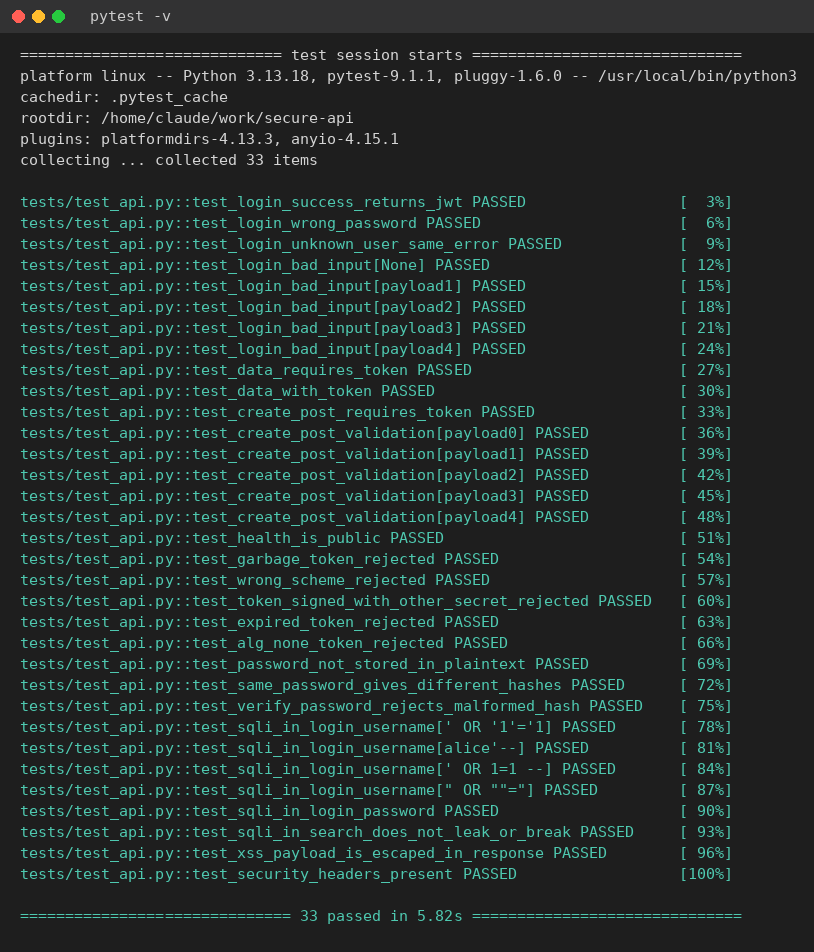
\includegraphics[width=\textwidth]{../docs/screenshots/pytest.png}
\caption{Результат запуска \code{pytest -v}: 33 теста пройдены}
\end{figure}

Ручная проверка через curl (скрипт \code{scripts/demo.sh}): без токена доступ запрещён (401), неверный пароль даёт 401,
верный --- выдаёт JWT, с токеном данные доступны, XSS-нагрузка экранируется, SQL-инъекция в параметре \code{q} не даёт
результата, поддельный токен отклоняется.

\begin{figure}[H]
\centering
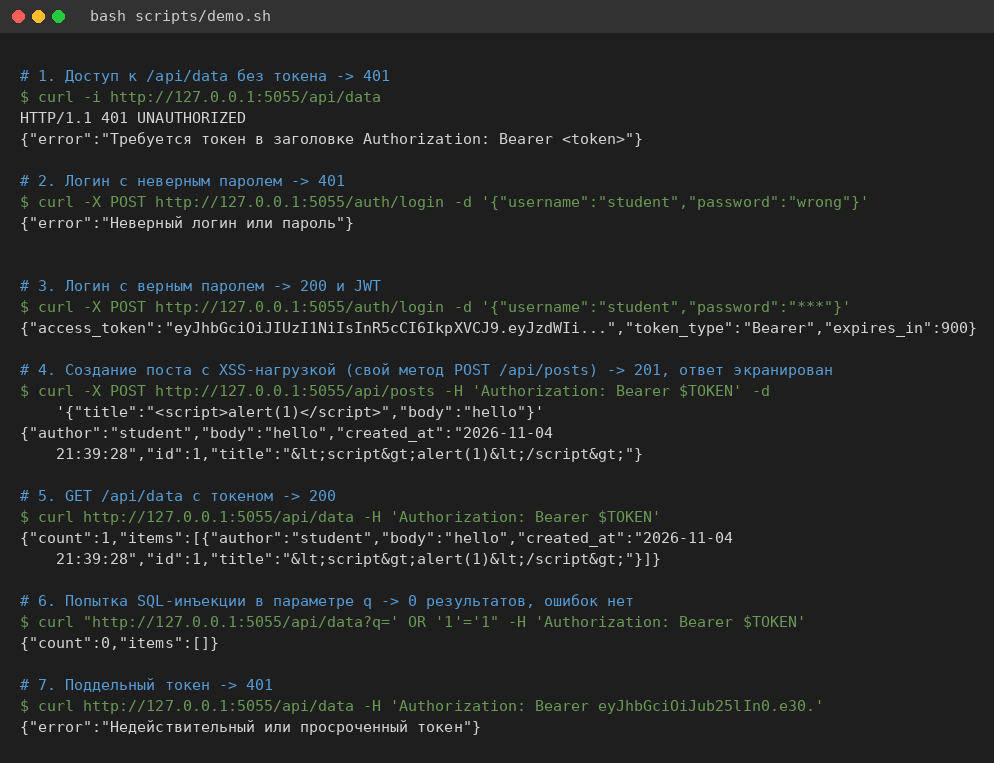
\includegraphics[width=\textwidth]{../docs/screenshots/curl_demo.png}
\caption{Проверка API через curl}
\end{figure}

\section{Отчёты SAST/SCA}
\begin{figure}[H]
\centering
\fbox{\parbox{0.9\textwidth}{\centering\vspace{2em}
Скриншот отчёта bandit (job \code{sast}) из GitHub Actions\vspace{2em}}}
\caption{SAST: bandit --- критических находок нет}
\end{figure}

\begin{figure}[H]
\centering
\fbox{\parbox{0.9\textwidth}{\centering\vspace{2em}
Скриншот отчёта pip-audit (job \code{sca}) из GitHub Actions\vspace{2em}}}
\caption{SCA: pip-audit --- известных уязвимостей в зависимостях нет}
\end{figure}

\section{Ответы на контрольные вопросы}

\paragraph{1. Почему bcrypt предпочтительнее SHA-256 для хэширования паролей?}
SHA-256 создан быть быстрым: на видеокарте можно перебирать миллиарды хэшей в секунду, поэтому утёкшую базу быстро
вскрывают подбором и радужными таблицами. bcrypt (как scrypt и Argon2) намеренно медленный и настраиваемый: параметр
стоимости можно повышать по мере роста мощности железа, соль встроена в формат и уникальна для каждого пароля, а scrypt и
Argon2 ещё и требуют много памяти, что затрудняет атаку на GPU и ASIC. В работе использован scrypt.

\paragraph{2. Чем SAST отличается от DAST?}
SAST (статический анализ) проверяет исходный код или зависимости без запуска программы, находит проблемы рано и указывает
строку кода, но даёт ложные срабатывания и не видит проблем окружения. DAST (динамический анализ) тестирует уже запущенное
приложение снаружи, имитируя атакующего (например, OWASP ZAP), находит реальные проблемы конфигурации и работы, но не
указывает место в коде и требует работающего стенда.

\paragraph{3. Как работает JWT?}
JWT состоит из трёх частей в Base64URL, разделённых точками: заголовок (алгоритм подписи, тип), полезная нагрузка (claims:
идентификатор пользователя, срок действия \code{exp}, издатель \code{iss} и др.) и подпись. Подпись --- это HMAC (или
асимметричная подпись) от заголовка и нагрузки с секретным ключом сервера. Сервер при получении токена пересчитывает подпись
своим ключом и сравнивает с переданной, а также проверяет срок действия, издателя и допустимый алгоритм; при изменении
любой части токена подпись не совпадёт. Нагрузка не шифруется, поэтому секретные данные в ней хранить нельзя.

\paragraph{4. Какие риски возникают без аудита сторонних библиотек?}
Зависимости составляют основную часть кода приложения, и в них регулярно находят уязвимости (например, RCE или обход
аутентификации). Без аудита такие уязвимости остаются в продукте незамеченными и эксплуатируются атакующими; возможны также
атаки на цепочку поставок (подменённые или вредоносные пакеты, typosquatting), лицензионные риски и использование
заброшенных библиотек без исправлений. Автоматический SCA в CI позволяет узнавать об этом сразу при каждом изменении.

\section*{Вывод}
Разработан REST API на Flask с аутентификацией по JWT, хэшированием паролей scrypt, защитой от SQL-инъекций и XSS.
Реализован pipeline GitHub Actions, который при каждом push и pull request запускает тесты, статический анализ (bandit) и
проверку зависимостей (pip-audit, OWASP Dependency-Check).

\end{document}
